\documentclass[sigconf, noacm = true, 11pt]{acmart}

\acmConference[]{Parallel Processing}{CIS 631}{Fall 2020}
\settopmatter{printfolios=true}
\settopmatter{printacmref=false} % Removes citation information below abstract
\renewcommand\footnotetextcopyrightpermission[1]{} % removes footnote with conference information in first column
% \pagestyle{plain} % removes running headers

%%
%% \BibTeX command to typeset BibTeX logo in the docs
\AtBeginDocument{%
  \providecommand\BibTeX{{%
    \normalfont B\kern-0.5em{\scshape i\kern-0.25em b}\kern-0.8em\TeX}}}

\newenvironment{tightItemize}{
\begin{itemize}
        \setlength{\itemsep}{1pt}
        \setlength{\parskip}{0pt}
        \setlength{\parsep}{0pt}
}{\end{itemize}
}

\usepackage{graphicx}
\usepackage{svg}
\usepackage{minted}
\usemintedstyle{bw}


\usepackage[ruled,vlined]{algorithm2e}

\usepackage{multirow}
\usepackage{multicol}

\usepackage{tikz} % To generate the plot from csv
\usepackage{pgfplots}

%%
%% end of the preamble, start of the body of the document source.
\begin{document}

%%
%% The "title" command has an optional parameter,
%% allowing the author to define a "short title" to be used in page headers.
\title{Parallel Game Tree Search: Gomoku}

%%
%% The "author" command and its associated commands are used to define
%% the authors and their affiliations.
%% Of note is the shared affiliation of the first two authors, and the
%% "authornote" and "authornotemark" commands
%% used to denote shared contribution to the research.
\author{Yuya Kawakami}

\affiliation{%
  \institution{University of Oregon}
\city{Eugene}
  \state{Oregon}
}
\email{ykawakam@uoregon.edu}
\author{Haoran Wang}
\affiliation{%
  \institution{University of Oregon}
\city{Eugene}
  \state{Oregon}
}
\email{hwang8@uoregon.edu}




%%
%% The abstract is a short summary of the work to be presented in the
%% article.
\begin{abstract}
With this work, we present parallel implementations of a game tree search algorithm called minimax using OpenMP and CUDA. The minimax algorithm is a recursive function used in game theory to find optimal moves for a player in information-perfect zero-sum games. This works looks specifically at the minimax algorithm for Gomoku, a popular board game played on a square sized board with black/white stones. Using the serial CPU implementation as our baseline, we found up to 100x speedup by leveraging GPUs. 

\end{abstract}

\maketitle
% \pagestyle{plain}

\section{Introduction}
\label{sec:intro}
Gomoku, also known as Five-in-a-row, originated from Japan and is very popular around the world. Two players put Go pieces (black and white stones) strategically on square size board, usually 15x15 or 19x19. The objective for any player is to have 5 pieces in a row. Figure~\ref{fig:board} is an example of what a Gomoku board may look like. Due to the two player zero-sum nature of the game, we can effectively leverage a game tree search algorithm like the minimax algorithm.\\
\\
For clarity sake, we will elaborate on what a game tree is and what it represents. In essence, a game tree is a directed graph where in which the nodes represent different board states and the edges represents move that a player can take from that given board state. Figure~\ref{fig:gametree} is an example of a game tree. The root node represents the initial board state and all its children are the potential next board state and so on and so forth. We use tic-tac-toe as an example here but the structure and idea is the same regardless of the game. The term depth is used for game trees in the same way as with graphs -  the distance between the leaf and root nodes. Hence, the game tree of Figure~\ref{fig:gametree} is of depth=2.\\
\\
In discussing Gomoku's game tree search, we will also touch on the complexity of we are trying to accomplish. The term \textit{complexity} in the context of games denote two different measures, \textit{state-space complexity} and \textit{game-tree complexity}. State-space complexity refers to the number of legal game positions reachable from the initial positions of the game. This contrasts with game-tree complexity which is defined as the number of leaf nodes in the solution search tree from the initial board state. \cite{allis_1994} As Allis writes, the game-tree complexity is what determines the size of minimax search tree needed to completely solve the game. Allis also includes Figure~\ref{fig:complexity} that shows the relative estimated game complexities. Notice that Gomoku, third from the right, is among the most complex games with a game-tree complexity of around $10^{80}$. In comparison, games like Othello with $10^{30}$ possible leaf nodes and chess with $10^{60}$ possible leaf nodes are relatively less complex. However, Go, the game from which Gomoku originates, is known to be the one of the most complex games with $10^{170}$ leaf nodes. It should be noted here that Allis estimates Gomoku's complexity with a 15x15 board and this will drastically change with a different sized board.\\

\begin{figure}[ht]
    \centering
    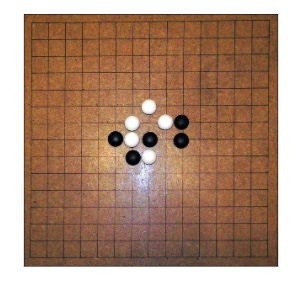
\includegraphics[scale=0.5]{images/gomoku_board.png}
    \caption{An example gomoku board}
    \label{fig:board}
\end{figure}

\begin{figure}[ht]
    \centering
    
\includegraphics[scale=0.40]{images/gametree.png}
    \caption{An example game tree}
    \label{fig:gametree}
\end{figure}


\begin{figure}[ht]
    \centering
    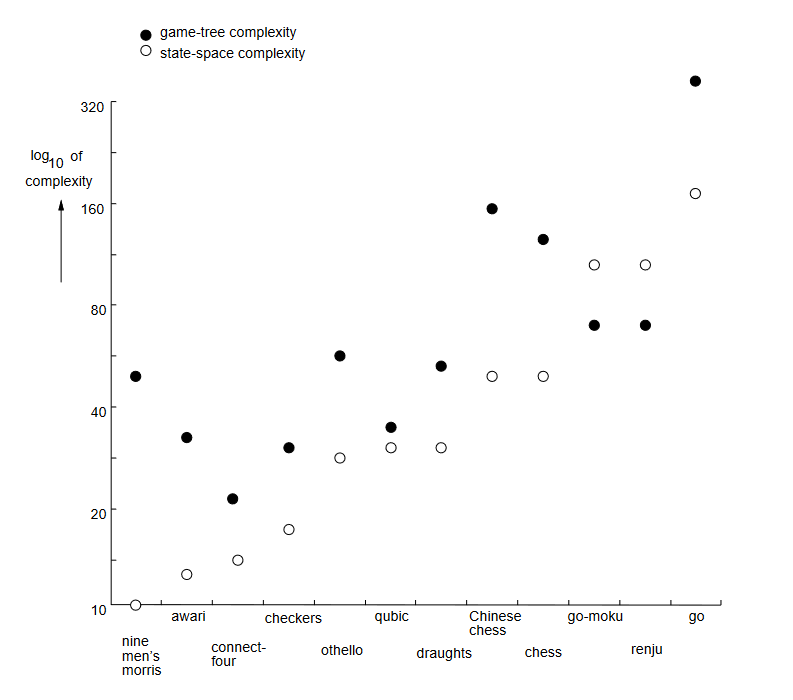
\includegraphics[scale=0.58]{images/complexity.PNG}
    \caption{Estimated game complexities \cite{allis_1994}}
    \label{fig:complexity}
\end{figure}

\noindent
Now, if there were a technology that could search through all $10^{80}$ leaf nodes, then we would be able to exactly calculate the best next move. However, exhaustively searching through all leaf nodes to determine the best move is infeasible and unrealistic. Therefore, we limit the size of the game tree by its depth. That is, we search the game tree up to some depth $d$ and determine the best move from that smaller game tree. Naturally, there is a trade-off between, $d$ and the how 'good' our best move is and this is an especially important consideration because our game tree increases exponentially in size as we increase the search depth. A larger tree would give us more information to determine the best move, but at the same time, would take much longer. One way to reduce the number of leaf nodes that we have to explore is through branch pruning and this can be done via alpha-beta pruning. (To be explained in Section~\ref{sec:minimax}). However, branch pruning alone proves to be insufficient if we are to search at a larger depth. The motivation of a parallel implementation is to improve on the computation time so that we are able to increase our search space without sacrificing accuracy. With this work, we present parallel implementations of Gomoku's game tree search using OpenMP, CUDA and other optimizations that we implemented.\\


\section{Minimax Algorithm}
\label{sec:minimax}
\subsection{Minimax}
Minimax is a backtracking algorithm that is used to find the optimal move for a player in a zero-sum game. The two players are called maximizer and minimizer. The goal of the maximizer is to get the highest score possible while the goal of the minimizer is to do the opposite and get the lowest score possible. The first step of minimax algorithm is to build a game tree to search.\\
\\
For a gomoku game tree, each node represents a board state that has a value associated with it. This value is the score of that specific board state, calculated by a scoring function with the heuristics based on stone shapes. Stone shape considers two parts, the number of consecutive stones and the number of open ends. If there are two open ends, it is called live; otherwise, it is called dead. Therefore, there are 7 categories of stone shapes: five in a row, live four, dead four, live three, dead three, live two, dead two. Five in a row has the highest score, while dead two has the lowest score.\\
\\
The pseudo code of minimax is shown below. This is a recursive function, the base case is reached when the search depth has been reached or the game has ended.\\

\begin{algorithm}[!htbp]
\SetAlgoLined
\SetKwInOut{Input}{input}
\SetKwInOut{Output}{output}
\Input{node, depth, maximizingPlayer}
\Output{score}

\If{depth == 0 or node is a terminal node}{
    return the heuristic score of node\;
}
\eIf{maximizingPlayer}{
    value = -$\infty$\;
    \For{each child of node}{
        score = max(value, minimax(child, depth-1, false))\;
    }
    return score\;
}{
    score = $\infty$\;
    \For{each child of node}{
        score = max(value, minimax(child, depth-1, true))\;
    }
    return score\;
}
\caption{Minimax}
\label{alg:minimax}
\end{algorithm}


\subsection{Alpha-Beta Pruning}
Alpha-Beta is an optimization for minimax algorithm. It prunes the branches of the game tree that need not be searched because there already exists a better move. Alpha-Beta pruning gets its name from two bounds that are passed along during the calculation, which restrict the set of possible solutions based on the portion of the each tree that has already been seen.\\
\\
Alpha represents the maximum lower bound of possible solutions, and beta represents the minimum upper bound of possible solutions. To visualize, we can use a line to represent the possible solutions. Initially, alpha is set to be -$\infty$, and beta is set to be $\infty$. \\
\\
As the game tree is being searched, there will be more restrictions about the range of possible solutions based on the nodes it has already seen. The bounds will get closer and closer together.\\
\\
Finally, once alpha and beta no longer overlap \(\alpha\leq\beta\), we know that this node could never result in a solution path, so we may stop processing this node. Meaning, we will stop generating its children and move back to its parent node. This is shown in Figure~\ref{fig:alpha-beta}.\\

\begin{figure}[!htbp]
    \centering
    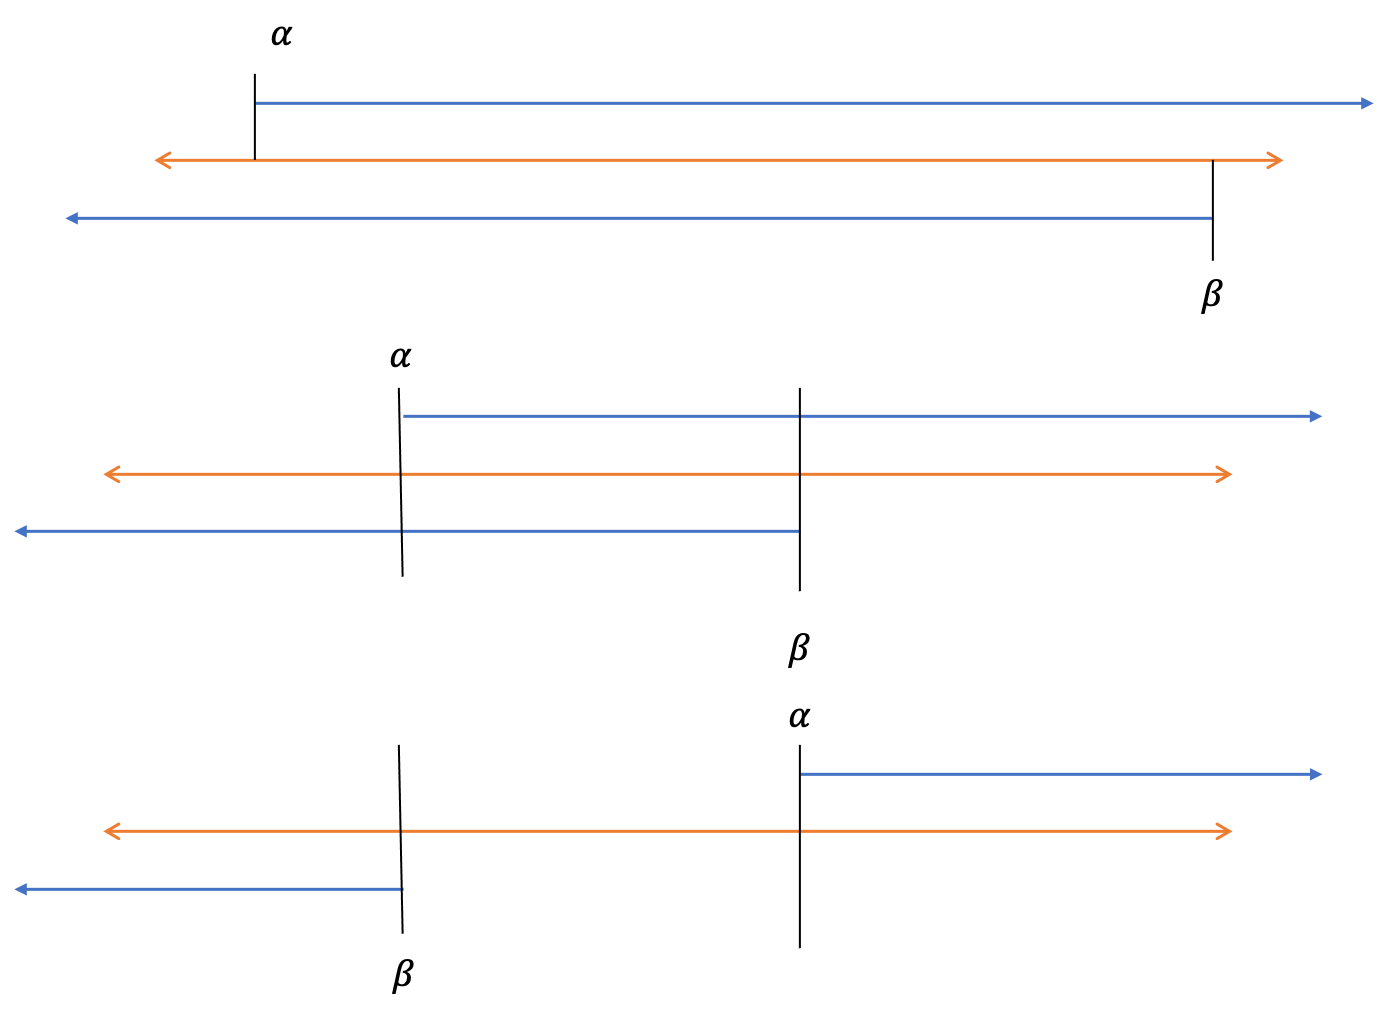
\includegraphics[scale=0.3]{images/ab.png}
    \caption{alpha and beta bounds}
    \label{fig:alpha-beta}
\end{figure}

\begin{algorithm}[!htbp]
\SetAlgoLined
\SetKwInOut{Input}{input}
\SetKwInOut{Output}{output}
\Input{node, depth, maximizingPlayer, alpha, beta}
\Output{score}

\If{depth == 0 or node is a terminal node}{
    return the heuristic score of node\;
}
\eIf{maximizingPlayer}{
    value = -$\infty$\;
    \For{each child of node}{
        score = max(value, minimax(child, depth-1, false, alpha, beta))\;
        alpha = max(alpha, score)\;
        \If{alpha $\leq$ beta}{
            break\;
        }{}
    }
    return score\;
}{
    score = $\infty$\;
    \For{each child of node}{
        score = max(value, minimax(child, depth-1, true, alpha, beta))\;
        beta = min(beta, score)\;
        \If{beta $\leq$ alpha}{
            break\;
        }{}
    }
    return score\;
}
\caption{Minimax with alpha-beta pruning}
\label{alg:minimaxab}
\end{algorithm}

\noindent
Algorithm~\ref{alg:minimaxab} is the pseudo code for the minimax algorithm with the inclusion of alpha-beta pruning. Note that the initial call to minimax with alpha-beta pruning sets alpha and beta to $-\infty$ and $+\infty$ respectively.


\subsection{Calculating the Best Move}
With the minimax algorithm and alpha-beta pruning defined, we can use this to find the best move as follows. For a given initial board state $s$, we first gather all the possible moves that the current player. For this work, we have defined all possible moves to be any unoccupied board location. Alternatively, we could only consider a subset by choosing positions that are adjacent, either above, below or diagonally, to an already occupied board location. Next, for each one of those moves we can call Algorithm~\ref{alg:minimax} and yield a score for each potential move. Finally, the move  with the highest score can be returned as the best move. In the case that there are multiple moves with the highest score, any of those would suffice as the 'best' move. 

\section{Related Works}
\label{sec:relworks}
There has been several previous and related works that attempted to parallelize and improve on serial implementations of the aforementioned minimax algorithm.\cite{borovska} \cite{Rocki} \cite{Mandadi}.\\
\\
Rocki and Suda explored CUDA-implemented parallel minimax tree search for Othello. This work was particularly important for this work as it highlighted some of the challenges of naive GPU implementations like thread divergence. Optimizations to the naive implementation that they propose like the sequential-parallel CUDA search are included in this work and will be explained further in detail in Section~\ref{sec:gpu}. \cite{Rocki}\\
\\
Borovska and Lazarova similarly explored parallel implementations of the minimax algorithm, but for tic-tac-toe. However, the parallelism that they expose is slightly different compared to Rocki and Suda and they describe them as \textit{partitioning at width} and \textit{partitioning at depth}, where \textit{partitioning at width} describes Rocki and Suda's approach and \textit{partitioning at depth} describes Borovska and Lazarova's approach. Figure~\ref{fig:widthvdepth} graphically shows the distinction that they draw. The \textit{partitioning at width} approach that Rocki and Suda take is to simply assign the search tree and assign them to multiple processors/threads for processing. The \textit{partitioning at width} approach that Borovska and Lazarova take is an attempt to leverage parallelism while keeping the benefits of alpha-beta pruning alive by instead parallelizing the move evaluation at each depth. They implement this with MPI and achieves around 2x speedup compared to serial code. It should be noted here though that tic-tac-toe is significantly less complex as a game compared to Gomoku. The PVS CUDA implementation described in Section~\ref{sec:gpu} will build off of this parallelization strategy.\cite{borovska}.


\begin{figure}[!htbp]
    \centering
    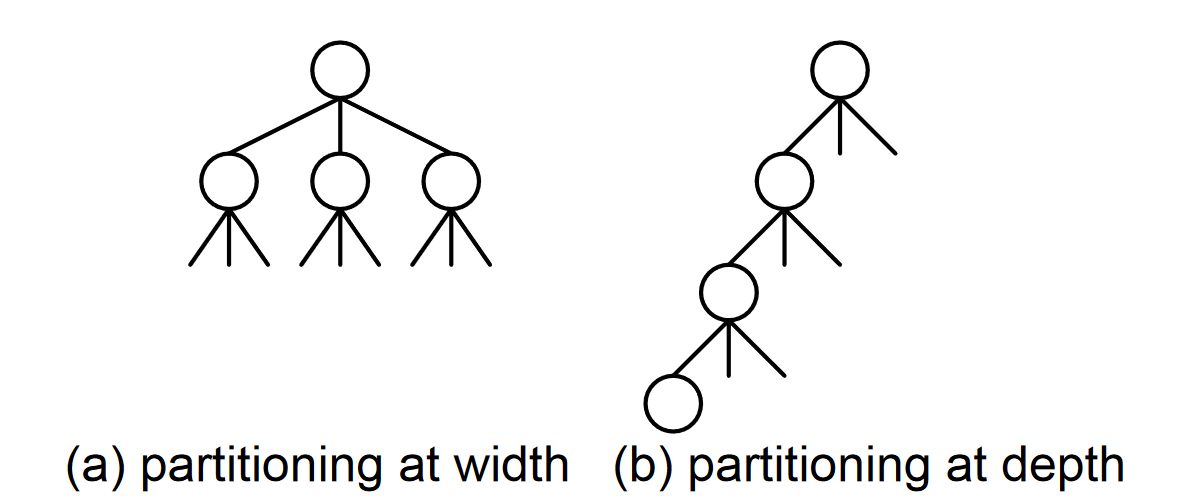
\includegraphics[scale=0.3]{images/relwork1.PNG}
    \caption{Partitioning at width vs depth}
    \label{fig:widthvdepth}
\end{figure}




\section{CPU Implementations}
\label{sec:cpu}
For CPU implementations we explore two options: 1) serial, 2) OpenMP parallelized version. As explained in Section~\ref{sec:minimax}, finding the best move is fairly trivial once the minimax algorithm is well defined. Since we have a for loop that can parallelized, (i.e. no data dependency between the sub-trees etc.) the OpenMP implementation simply adds a \mintinline{C}{#pragma omp parallel for} on the for loop. Although it's simplicity is attractive, this strategy fails to take full advantage of alpha-beta bounds found in other sub-trees. This is a similar criticism that Borovska and Lazorova had as explained in Section~\ref{sec:relworks}.~\cite{borovska}. 

\begin{algorithm}[!htbp]
\SetAlgoLined
\SetKwInOut{Input}{input}
\SetKwInOut{Output}{output}
\Input{depth, currentPlayer}
\Output{bestScore}

bestScore = -$\infty$\\
\For{each possible child move for currentPlayer }{
        bestScore = max(bestScore, minimax-alpha-beta-pruning(child, depth-1, true, $-\infty$, $+\infty$))\;
    }
    return bestScore
\caption{getBestMove}
\label{alg:bestscore}
\end{algorithm}

\section{GPU Implementations}
\label{sec:gpu}
\subsection{Naive CUDA}

One simple way to implement CUDA parallel minimax is to launch CUDA threads to each potential move from the initial board state. Suppose we have a 15x15 board and lets assume that player 1 has played one move. Then, player 2 has $15\cdot 15-1=224$ potential moves from which to choose the optimal move. We can then launch 1 thread block of dimension \mintinline{C}{(224,1,1)} and have each thread of that block explore every potential move. \\
\\
As we will demonstrate in Section~\ref{sec:results}, this method severely underperforms in comparison to the CPU implementations for a couple of reasons, especially at higher search depths. The first is related to how our heuristic function is defined. Recall from Section~\ref{sec:minimax} that a static evaluation is calculated whenever the minimax algorithm encounters a terminal node or when the depth is equal to 0, signalling that we have gone as far as we want in the search tree. The heuristic function inevitably contains many if-else statements to account for different board configurations and states. Since in CUDA threads are run at the granularity of warps and since CUDA requires that each thread in a warp execute the same operation, this set of conditional operations causes thread divergence within the warp. This, of course, leads to sub-optimal performance from the GPU. \\
\\
Furthermore, and perhaps most importantly, 224 threads simply is not enough threads to see performance gains in CUDA. To extract good performance from the GPU, we need to use a thousands or tens of thousands of threads to hide latency and increase the chance of keeping the GPU busy. This second limitation of the naive GPU implementation motivates the sequential-parallel approach explained next.

\subsection{Sequential-parallel CUDA}
As mentioned the sequential-parallel CUDA implementation is an attempt to overcome the second limitation in the naive CUDA implementation. The main idea of this approach is to launch as many lightweight threads as possible. To this end, the sequential-parallel approach first splits the search tree of depth $d$ into two parts:
an upper part of depth $s$ and a lower part of depth $p$, where the upper part will be searched sequentially and the lower part will be searched in parallel. Note that $d=s+p$ must hold true. The lower part is then is divided into $k$ sub-trees and a GPU thread is launched for each of these $k$ sub-trees. Figure~\ref{fig:seqpar} provides graphic aid for the tree splitting.\\
\\
Now with this setup, the game tree search process takes 3 steps. \cite{Rocki}
\begin{enumerate}
    \item From the root node, sequentially search through depth $s$ and store the leaf board state into an array 
    \item For each of the leaves/board states, execute a parallel search of depth $p$.
    \item Traverse down the upper section of the tree retrieving the results from step 2 and finally return the best move.
\end{enumerate}

\begin{figure}[!htbp]
    \centering
    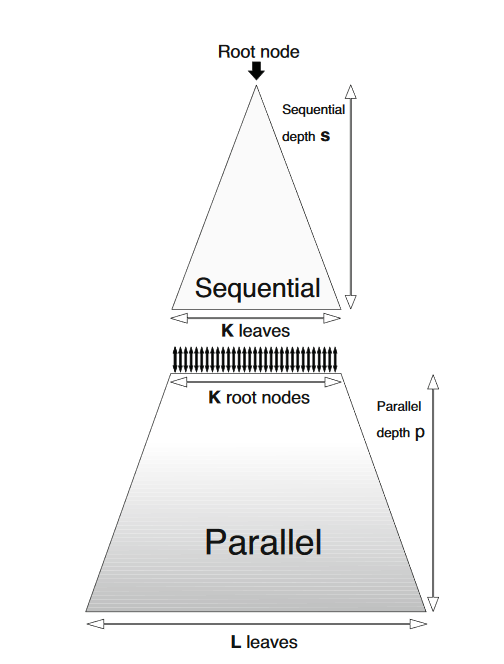
\includegraphics[scale=0.45]{images/seqpar.PNG}
    \caption{Parallelization strategy for sequential-parallel CUDA \cite{Rocki}}
    \label{fig:seqpar}
\end{figure}

\noindent
Since the original goal with the sequential-parallel method was to launch more lightweight threads, we can compare this method to the naive method with an example. Suppose again that we have a board of size 15x15 and player 1 has played one move. In the naive implementation, as explained in the previous section, we would launch 224 threads, each to explore some depth $d$. Note that the number of threads launched in the naive version is independent on $d$. Now suppose we set $d=3$ and we set $s=2, p=1$. This means we are exploring depth of 2 sequentially, and depth of 1 in parallel. In this scenario, we would instead launch $224\cdot 223=49952$ threads. As we can see, this is more in line with the general CUDA practice of launching more lightweight threads. In the sequential-parallel method, each GPU thread is responsible of depth of 1, whereas in the naive implementation each GPU thread would have been tasked with exploring a depth of 3 on its own. The difference in amount of work delegated to each thread, compounded with the effects of thread divergence as well, the sequential-parallel implementation leads to significant improvement compared to the naive implementation.\\
\\
One limitation/consideration that Rocki and Suda mention in their paper is that this strategy brings an overhead of having to execute the sequential tree section twice, once to populate the list of possible board states and once to retrieve the scores after the GPU threads calculate the scores.~\cite{Rocki} They further remark that due to this overhead, the choice of $s$ is important so that we can decrease the cost of this redundant operation, while generating enough leaves to saturate the GPU and its resources.




\subsection{PVS CUDA}
The problem with naive and the sequential-parallel CUDA implementation is that the result from earlier branches are used to determine whether later branches should be examined or not. If we search multiple branches in parallel, those branches do not have the bounds from each other to work with. This will result in searching unnecessary branches that will not lead to a solution. Therefore, we optimized our CUDA implementation by using PVS method from this paper \cite{pvsgpu}.\\

\noindent
Principle Variation Search (PVS) \cite{pvs} is a refinement of the alpha-beta pruning technique. The core idea is to assume the first examined move is the best and try to determine if a sub-tree will lead a cutoff. Before traversing through the tree further, a null-window search of the corresponding sub-tree is performed first. Null-window search means that the $\alpha$ and $\beta$ bounds are set to $\alpha = \alpha$ and $\beta = \alpha + 1$. Even if that means that the search will always fail, we will be able to determine if the earch will cause a $\beta$ cutoff or lies under $\alpha$ instead. If it fails, the sub-tree does not need to be searched any further, otherwise the sub-tree will be searched again with the result of the null-window search. The pseudo code of PVS is shown below.\\

\begin{algorithm}[!htbp]
\SetAlgoLined
\SetKwInOut{Input}{input}
\SetKwInOut{Output}{output}
\Input{nodes, $\alpha$, $\beta$, depth}
\Output{score}
\If{depth == 0}{
    return evaluate(n)\;
}
nodes = generate(n)\;
\If{nodes.isEmpty()}{
    return evalute(n)\;
}
score = PVS(nodes[0], $\beta$, $\alpha$, depth-1)\;
\For{j = 1 \KwTo nodes.size()-1}{
    \If{score $\geq$ $\beta$}{
        break\;
    }
    $\alpha$ = max(score, $\alpha$)\;
    value = PVS(nodes[j], $\alpha-1$, $\alpha$, depth-1)\;
    \If{value $>$ score}{
        \eIf{$\alpha$ $<$ value \& value $<$ $\beta$ \& depth $>$ 2}{
            score = PVS(nodes[j], $\beta$, value, depth-1)\;
        }{
            score = value\;
        }
    }
}
return score\;
\caption{PVS}
\label{alg:PVS}
\end{algorithm}

\noindent
This paper \cite{pvsgpu} has shown a hybrid approach of using both CPU and GPU. The leftmost branch is searched on the CPU, then the remaining child nodes will be searched on the GPU. This allows the GPU branches to use the bounds from CPU branch to avoid searching branches that would otherwise be pruned in serial implementation. Then we assign one block for each child node to search down the sub-tree rooted at the child node.\\

\begin{figure}[!htbp]
    \centering
    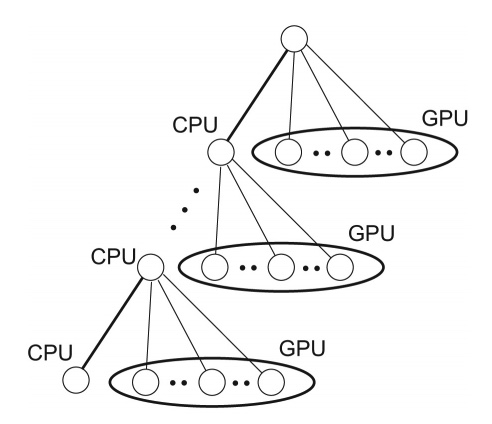
\includegraphics[scale=0.4]{images/pvs.jpg}
    \caption{CPU establishes bounds for GPU\cite{pvsgpu}}
\end{figure}

\begin{figure}[!htbp]
    \centering
    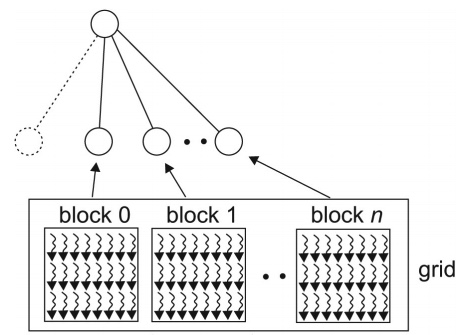
\includegraphics[scale=0.4]{images/pvs2.jpg}
    \caption{One block per child node\cite{pvsgpu}}
\end{figure}

\subsection{Dynamic Parallelism CUDA}
One problem with our PVS implementation is that we uses one block to fully search the entire sub-tree rooted at a child node. As depth increases, each block needs to search increasingly larger sub-trees. Therefore, we seek to fully parallelize our game tree search by using dynamic parallelism. \cite{dp}\\
\\
Dynamic Parallelism is a feature added in CUDA 5.0. It enables a CUDA kernel to create and synchronize new nested work, using the CUDA runtime API to launch other kernels, synchronize on kernel completion and perform device memory management, all without CPU involvement. \cite{dp2}\\
\\
In our implementation, our \textit{cudaSearchKernel} kernel function launches new kernels for each node to be searched. However, one possible trade off of this approach is the overhead of launching so many kernels.\\


\section{Experimental Design}
\label{sec:expdesign}
\subsection{Experiments}
We did two type of experiments:
\begin{itemize}
    \item We tested how long it takes computer to calculate the best move given a input move. This is experiment is done for all methods we implemented.
    \item We tested how long it takes computer to complete a whole game. We only tested this on PVS and Dynamic CUDA, due to limited computing resources.
\end{itemize}

\subsection{Experiment Setup}
We tested our CPU code on department's ix server. It has two sockets with AMD Opteron 6376 on each socket. Each CPU has 8 cores, 16 threads. So, there are 32 hardware threads in total. We tested our GPU code on Google Cloud Computing Instance that has a Tesla V100 GPU, with 16GB of HBM2 memory, 900GB/sec memory bandwidth.

\subsection{Testing for Correctness}
The lack of a clear or correct answer made testing for correctness slightly harder than other algorithms as the 'best' move depends entirely on the heuristic function and there is no publicly available benchmark to verify our algorithm. In place of these checks for this work, we have instead compared any parallel/optimized code against the original serial CPU version to ensure that they return the same results. 

\section{Results}
\label{sec:results}
This section shows the results from our experiments as well as analysis for the performance.

\subsection{Serial}
This table below shows the result for our serial implementation. Time is measured in seconds.
\begin{table}[!htbp]
\centering
\begin{tabular}{|c|c|c|c|c|} 
\hline
\multirow{2}{*}{Board dimension} & \multicolumn{4}{c|}{Search Depth}     \\ 
\cline{2-5}
                                 & 1       & 2      & 3       & 4        \\ 
\hline
6x6                              & 0.00019 & 0.0051 & 0.0292  & 0.272    \\ 
\hline
9x9                              & 0.00069 & 0.0269 & 0.4572  & 12.669   \\ 
\hline
12x12                            & 0.00184 & 0.1324 & 4.6165  & 271.388  \\ 
\hline
15x15                            & 0.00415 & 0.4375 & 29.651  & -        \\ 
\hline
18x18                            & 0.00874 & 1.1842 & 158.13  & -        \\ 
\hline
21x21                            & 0.01346 & 2.8423 & 571.07  & -        \\ 
\hline
24x24                            & 0.01722 & 6.8895 & 1718.01 & -        \\
\hline
\end{tabular}
\caption{Serial Result}
\end{table}

\noindent
Our serial implementation definitely suffers with larger board size and deeper depth. Due to limited computing resources, we were not able to run board size larger than 12x12 at depth 4.

\subsection{OpenMP}
This table below shows the result for our OpenMP solution, using 32 threads. Time is measured in seconds. 
\begin{table}[!htbp]
\centering
\begin{tabular}{|c|c|c|c|c|} 
\hline
\multirow{2}{*}{Board dimension} & \multicolumn{4}{c|}{Search Depth}     \\ 
\cline{2-5}
                                 & 1       & 2      & 3       & 4        \\ 
\hline
6x6                              & 0.0083 & 0.009 & 0.01    & 0.03    \\ 
\hline
9x9                              & 0.0086 & 0.009 & 0.05    & 2.712   \\ 
\hline
12x12                            & 0.0067 & 0.027 & 0.42    & 56.947  \\ 
\hline
15x15                            & 0.0075 & 0.036 & 2.62    & -        \\ 
\hline
18x18                            & 0.0065 & 0.077 & 13.21   & -        \\ 
\hline
21x21                            & 0.0082 & 0.17  & 109.87  & -        \\ 
\hline
24x24                            & 0.0075 & 0.41  & 358.98  & -        \\
\hline
\end{tabular}
\caption{OpenMP Result}
\end{table}

\noindent
Our OpenMP solution performs worse than the serial implementation when the boards size is smaller than 12x12 and depth is less than 2; Our OpenMP solution achieves good speedup, up to ~16x when the board size is larger than 21x21 and depth = 2. However, even with OpenMP, it still took too long to run board size larger than 15 at depth = 4. The figure  below shows the speedup factor on a logarithmic scale ($\log_{10}$) for different board size at depth = 1, 2, 3, 4 compared to the serial implementation\\

\begin{tikzpicture}[scale=0.8]
\begin{axis}[
        title = {OpenMP: Speedup on a Logarithmic Scale},
		xlabel=Depth,
		xtick={1,2,3,4},
		ylabel=$\log_{10}$ of Speedup Factor,
		legend pos=outer north east]
    \addplot table {./data/omp6.dat};
    \addplot table {./data/omp9.dat};
    \addplot table {./data/omp12.dat};
    \addplot table {./data/omp15.dat};
    \addplot table {./data/omp18.dat};
    \addplot table {./data/omp21.dat};
    \addplot table {./data/omp24.dat};
    \addlegendentry{$6x6$};
    \addlegendentry{$9x9$};
    \addlegendentry{$12x12$};
    \addlegendentry{$15x15$};
    \addlegendentry{$18x18$};
    \addlegendentry{$21x21$};
    \addlegendentry{$24x24$};
	\end{axis}
\end{tikzpicture}

\subsection{Naive CUDA}
This table below shows the result for our Naive CUDA solution. Time is measured in seconds.
\begin{table}[!htbp]
\centering
\begin{tabular}{|c|c|c|c|c|} 
\hline
\multirow{2}{*}{Board dimension} & \multicolumn{4}{c|}{Search Depth}     \\ 
\cline{2-5}
                                 & 1       & 2      & 3       & 4        \\ 
\hline
6x6                              & 0.079   & 0.093 & 0.268  & 17.051    \\ 
\hline
9x9                              & 0.08    & 0.117 & 2.906  & -   \\ 
\hline
12x12                            & 0.082   & 0.184 & 29.96 & -  \\ 
\hline
15x15                            & 0.082   & 0.258 & -      & -        \\ 
\hline
18x18                            & 0.081   & 0.342 & -      & -        \\ 
\hline
21x21                            & 0.082   & 0.545 & -      & -        \\ 
\hline
24x24                            & 0.083   & 0.891 & -      & -        \\
\hline
\end{tabular}
\caption{Naive CUDA}
\end{table}

\noindent
Our Naive CUDA implementation achieved up to 7x speedup for board size larger than 15x15 at depth = 2. However, it did not achieve the same level of speedup as OpenMP did. In addition, it has memory issues when we try to run larger board size at depth 3 and 4. The limitations of the Naive CUDA implementation that were laid out in Section~\ref{sec:gpu} are shown here.\\

\subsection{Sequential-Parallel CUDA}
This table below shows the result for our Sequential Parallel CUDA solution, using 768 threads per block. Time is measured in seconds.

\begin{table}[!htbp]
\centering
\begin{tabular}{|c|c|c|c|c|} 
\hline
\multirow{2}{*}{Board dimension} & \multicolumn{4}{c|}{(total depth, sequential depth)}     \\ 
\cline{2-5}
                                 & (2,1)       & (3,2)      & (4.2)       & (4,3)        \\ 
\hline
6x6                              & 0.010   & 0.037 & 0.577  & 0.550    \\ 
\hline
9x9                              & 0.037    & 0.292 & 67.37  & 13.77   \\ 
\hline
12x12                            & 0.119   & 1.728 & 1999.45 & 131.92  \\ 
\hline
15x15                            & 0.193   & 6.649 & -      & -        \\ 
\hline
18x18                            & 0.310   & 11.66 & -      & -        \\ 
\hline
21x21                            & 0.573   & 31.72 & -      & -        \\ 
\hline
24x24                            & 0.868   & - & -      & -        \\
\hline
\end{tabular}
\caption{Sequential Parallel CUDA}
\end{table}

\noindent
Our Sequential Parallel CUDA achieved steady speedup at depth = 3, and it achieved speedup up to \textasciitilde{31}x at depth = 4 for board size 6x6. The figure  below shows the speedup factor on a logarithmic scale ($\log_{10}$) for different board size at depth = 2, 3, 4 against Naive CUDA.\\ 
\\
Due to the current implementation, the sequential-parallel implementation runs into memory issues at large board size and large depth. This is primarily due to the fact that we have to keep track of all the leaf nodes from the sequential step. Recall from Section~\ref{sec:gpu} that this implementation stores each board state that the sequential step produces. For total depth=4 and sequential depth=3, at board 15x15, we are storing up to $224*223*222=11,089,344$ integers just in the first step. With other necessary allocations, this method quickly runs of GPU memory. Another important comparison to note here is the difference between the (4,2) and (4,3) setup. As evident from our results, we find that our performance degrades substantially moving from a sequential depth of 3 to 2. This is due to warp divergence that was mentioned in Section~\ref{sec:gpu} as a limitation of the current CUDA heuristic function. Compared to naive CPU, The below compared the speedup to naive CUDA. Note that some data is missing due to naive CUDA taking too long to complete for some of sequential-parallel's counterparts. \\

\begin{tikzpicture}[scale=0.8]
\begin{axis}[
        title = {Sequential-parallel: Speedup on a Logarithmic Scale},
		xlabel=Depth,
		xtick={2,3,4},
		ylabel=$\log_{10}$ of Speedup Factor,
		legend pos=outer north east]
    \addplot table {./data/seq6.dat};
    \addplot table {./data/seq9.dat};
    \addplot table {./data/seq12.dat};
    \addplot table {./data/seq15.dat};
    \addplot table {./data/seq18.dat};
    \addplot table {./data/seq21.dat};
    \addplot table {./data/seq24.dat};
    \addlegendentry{$6x6$};
    \addlegendentry{$9x9$};
    \addlegendentry{$12x12$};
    \addlegendentry{$15x15$};
    \addlegendentry{$18x18$};
    \addlegendentry{$21x21$};
    \addlegendentry{$24x24$};
	\end{axis}
\end{tikzpicture}


\subsection{PVS CUDA}
This table below shows the result for our PVS CUDA solution, using 768 threads per block. Time is measured in seconds.\\
\begin{table}[!htbp]
\centering
\begin{tabular}{|c|c|c|c|c|} 
\hline
\multirow{2}{*}{Board dimension} & \multicolumn{4}{c|}{Search Depth}     \\ 
\cline{2-5}
                                 & 1       & 2      & 3       & 4        \\ 
\hline
6x6                              & 0.0045 & 0.013 & 0.086  & 0.199    \\ 
\hline
9x9                              & 0.0058 & 0.027 & 1.34   & 0.365   \\ 
\hline
12x12                            & 0.0062 & 0.012 & 5.56   & 2.845  \\ 
\hline
15x15                            & 0.0052 & 0.016 & 159.05 & 10.498        \\ 
\hline
18x18                            & 0.0061 & 0.025 & 161.88 & -        \\ 
\hline
21x21                            & 0.0069 & 0.037 & -      & -        \\ 
\hline
24x24                            & 0.0073 & 0.056 & -      & -        \\
\hline
\end{tabular}
\caption{PVS CUDA}
\end{table}

\noindent
Our PVS implementation achieves very good speedup against Naive CUDA implementation. It achieves steady speedup around \textasciitilde{17}x across all board size at depth = 1 and depth = 2, around \textasciitilde{3}x speedup at depth = 3. The figure  below shows the speedup factor on a logarithmic scale ($\log_{10}$) for different board size at depth = 1, 2, 3, 4 against Naive CUDA.\\

\begin{tikzpicture}[scale=0.8]
\begin{axis}[
        title = {PVS: Speedup on a Logarithmic Scale},
		xlabel=Depth,
		xtick={1,2,3,4},
		ylabel=$\log_{10}$ of Speedup Factor,
		legend pos=outer north east]
    \addplot table {./data/pvs6.dat};
    \addplot table {./data/pvs9.dat};
    \addplot table {./data/pvs12.dat};
    \addplot table {./data/pvs15.dat};
    \addplot table {./data/pvs18.dat};
    \addplot table {./data/pvs21.dat};
    \addplot table {./data/pvs24.dat};
    \addlegendentry{$6x6$};
    \addlegendentry{$9x9$};
    \addlegendentry{$12x12$};
    \addlegendentry{$15x15$};
    \addlegendentry{$18x18$};
    \addlegendentry{$21x21$};
    \addlegendentry{$24x24$};
	\end{axis}
\end{tikzpicture}

\subsection{Dynamic Parallelism CUDA}
This table below shows the result for our Dynamic Parallelism CUDA solution, using 768 threads per block. Time is measured in seconds.\\

\begin{table}[!htbp]
\centering
\begin{tabular}{|c|c|c|c|c|} 
\hline
\multirow{2}{*}{Board dimension} & \multicolumn{4}{c|}{Search Depth}     \\ 
\cline{2-5}
                                 & 1       & 2      & 3       & 4        \\ 
\hline
6x6                              & 0.0038 & 0.048 & 4.74  & -    \\ 
\hline
9x9                              & 0.0047 & 0.886 & 141.48  & -   \\ 
\hline
12x12                            & 0.0058 & 13.538 & -  & -  \\ 
\hline
15x15                            & 0.0081 & 29.12 & - & -        \\ 
\hline
18x18                            & 0.0094 & 36.92 & -  & -        \\ 
\hline
21x21                            & 0.0121 & - & -  & -        \\ 
\hline
24x24                            & 0.0147 & - & - & -        \\
\hline
\end{tabular}
\caption{Dynamic Parallelism CUDA}
\end{table}

\noindent
Our Dynamic Parallelism achieved good speedup against Naive CUDA implementation across all board size at depth = 1. However, it performed worse than naive CUDA at higher depth and larger board size.To find out the reason, we used \textit{nvprof} tool to see which part is taking the most time during the execution. For board size of 12x12, depth = 2, the result of nvprof report is shown below.\\

\begin{verbatim}
GPU activities:

Time     Calls Name
10.912us 6     [CUDA memcpy HtoD]
5.7920us 2     [CUDA memcpy DtoH]
3.3920us 2     [CUDA memset]

API Calls:

Time     Calls Name
12.4633s 8     cudaMemcpy
\end{verbatim}

\noindent
In \textit{nvprof}, section "GPU activities" lists activities which execute on the GPU, such as kernel, CUDA memcpy, CUDA memset. The timing information here represents the execution time on the GPU. Section "API calls" list CUDA Runtime/Driver API calls, the timing information here represents the execution time on the host. As shown above, cudaMemcpy takes overwhelming long time during the execution. This is the main reason for its slower performance than PVS.

\subsection{Overall Speedup Comparison}
The table below lists the speedup each method achieved for board size 15x15, and depth = 2. Except for the dynamic parallelism CUDA, we see performance improvements all across the board, peaking at 27x speedup for this configuration. Of the data that we collected (some configurations took too long / ran out of memory), the peak speedup was with board size 12x12 with depth=4 where the serial implementation took 271.388s and PVS CUDA took 2.845s resulting in a \textasciitilde{100}x speedup. 

\begin{table}[!htbp]
\begin{tabular}{|c|c|c|}
\hline
\textbf{Method} & \textbf{Time} & \textbf{Speedup} \\ \hline
Serial          & 0.4375        &                  \\ \hline
OpenMP          & 0.036         & 12.15x           \\ \hline
Naive           & 0.258         & 1.70x            \\ \hline
Sequential      & 0.193         & 2.27x            \\ \hline
PVS             & 0.016         & 27.34x           \\ \hline
Dynamic         & 29.12         & 0.02x            \\ \hline
\end{tabular}
\caption{Overall Speedup Comparison}
\end{table}


\subsection{Test a Whole Game}
The two tables below are the results to run a whole game for PVS and Dynamic CUDA, using 768 threads per block.\\

\begin{table}[!htbp]
\centering
\begin{tabular}{|c|c|c|c|c|} 
\hline
\multirow{2}{*}{Board dimension} & \multicolumn{4}{c|}{Search Depth}     \\ 
\cline{2-5}
                                 & 1       & 2      & 3       & 4        \\ 
\hline
6x6                              & 0.0138  & 0.11  & -  & -    \\ 
\hline
9x9                              & 0.015   & 0.60  & -  & -   \\ 
\hline
12x12                            & 0.016   & 1.54  & -  & -  \\ 
\hline
15x15                            & 0.020   & 10.85 & - & -        \\ 
\hline
18x18                            & 0.028   & 18.88 & -  & -        \\ 
\hline
21x21                            & 0.033   & 99.04 & -  & -        \\ 
\hline
24x24                            & 0.034   & -     & - & -        \\
\hline
\end{tabular}
\caption{PVS: automated game}
\end{table}

\begin{table}[!htbp]
\centering
\begin{tabular}{|c|c|c|c|c|} 
\hline
\multirow{2}{*}{Board dimension} & \multicolumn{4}{c|}{Search Depth}     \\ 
\cline{2-5}
                                 & 1       & 2      & 3       & 4        \\ 
\hline
6x6                              & 0.0238  & 0.349  & 24.921  & -    \\ 
\hline
9x9                              & 0.0306   & 7.618  & -  & -   \\ 
\hline
12x12                            & 0.0468   & 278.748  & -  & -  \\ 
\hline
15x15                            & 0.0718   & - & - & -        \\ 
\hline
18x18                            & 0.0998   & - & -  & -        \\ 
\hline
21x21                            & 0.145   & - & -  & -        \\ 
\hline
24x24                            & 0.178   & -     & - & -        \\
\hline
\end{tabular}
\caption{Dynamic: automated game}
\end{table}

\noindent
As the results shown, our PVS and Dynamic CUDA can only run on smaller problem size. 

\section{Conclusion and Future work}
\label{sec:conclusion}
Before we conclude, we will highlight some modifications that will improve the performance of our implementations, especially our GPU implementations. Currently, a board state is represented using an array with $width\cdot height$ number of integers. One major change and improvement is to adapt a bit-represented board to reduce memory usage and to adopt bitwise operations. Rocki and Suda reports a \textasciitilde10x speedup with this improvement.~\cite{Rocki} Since communication costs between GPU and CPU are high, we expect that we would also see significant performance improvement with this board representation.\\
\\
Thread divergence was one of the performance issues for our CUDA implementations. As such, methods that would reduce this like reducing if-else statements in favor of bitwise operations in our code should also greatly help our performance. Furthermore, Rocki and Suda also propose methods like branch reordering so that the search process starts a a branch with the largest number of children so that the threads within a warp can follow a similar execution flow as possible.\cite{Rocki}\\
\\
To sum, this work looked at several parallelization strategies for a minimax game tree search including OpenMP for CPU, Naive CUDA, Sequential-Parallel CUDA, PVS CUDA, and Dynamic Parallelism CUDA. While there are significant rooms for improvement, we nevertheless found impressive speedup with GPUs. Future work would apply, among others, improvements listed in this section and we suspect that the GPU performance gains will only increase as the board size and search depth increases. 




\newpage
%%
%% The next two lines define the bibliography style to be used, and
%% the bibliography file.
\bibliographystyle{ACM-Reference-Format}
\bibliography{report.bib}


\end{document}
\endinput
%%
%% End of file `sample-sigconf.tex'.
